\documentclass[paper=a4, fontsize=11pt]{scrartcl} % A4 paper and 11pt font size

\usepackage[T1]{fontenc} % Use 8-bit encoding that has 256 glyphs
\usepackage{fourier} % Use the Adobe Utopia font for the document - comment this line to return to the LaTeX default
\usepackage[english]{babel} % English language/hyphenation
\usepackage{amsmath,amsfonts,amsthm,amssymb} % Math packages

\usepackage{algorithm, algorithmic}
\renewcommand{\algorithmicrequire}{\textbf{Input:}} %Use Input in the format of Algorithm  
\renewcommand{\algorithmicensure}{\textbf{Output:}} %UseOutput in the format of Algorithm  

\usepackage{graphicx}
\usepackage{blindtext}
\usepackage{enumerate}
\usepackage{ulem} 
\usepackage{pdfpages}

\usepackage{listings}
\lstset{language=Matlab}

\usepackage{lipsum} % Used for inserting dummy 'Lorem ipsum' text into the template

\usepackage{sectsty} % Allows customizing section commands
\allsectionsfont{\centering \normalfont\scshape} % Make all sections centered, the default font and small caps

\usepackage{fancyhdr} % Custom headers and footers
\pagestyle{fancyplain} % Makes all pages in the document conform to the custom headers and footers
\fancyhead{} % No page header - if you want one, create it in the same way as the footers below
\fancyfoot[L]{} % Empty left footer
\fancyfoot[C]{} % Empty center footer
\fancyfoot[R]{\thepage} % Page numbering for right footer
\renewcommand{\headrulewidth}{0pt} % Remove header underlines
\renewcommand{\footrulewidth}{0pt} % Remove footer underlines
\setlength{\headheight}{13.6pt} % Customize the height of the header

\numberwithin{equation}{section} % Number equations within sections (i.e. 1.1, 1.2, 2.1, 2.2 instead of 1, 2, 3, 4)
\numberwithin{figure}{section} % Number figures within sections (i.e. 1.1, 1.2, 2.1, 2.2 instead of 1, 2, 3, 4)
\numberwithin{table}{section} % Number tables within sections (i.e. 1.1, 1.2, 2.1, 2.2 instead of 1, 2, 3, 4)

\setlength\parindent{0pt} % Removes all indentation from paragraphs - comment this line for an assignment with lots of text

\newcommand{\horrule}[1]{\rule{\linewidth}{#1}} % Create horizontal rule command with 1 argument of height
\newcommand*{\dif}{\mathop{}\!\mathrm{d}}

\title{	
\normalfont \normalsize 
\textsc{Shanghai Jiao Tong University, UM-SJTU JOINT INSTITUTE} \\ [25pt] % Your university, school and/or department name(s)
\horrule{0.5pt} \\[0.4cm] % Thin top horizontal rule
\huge Technical Communication\\ HW3 \\ % The assignment title
\horrule{2pt} \\[0.5cm] % Thick bottom horizontal rule
}

\author{Yu Cang \quad 018370210001} % Your name

\date{\normalsize \today} % Today's date or a custom date

\begin{document}

\maketitle % Print the title

\section{Mind Map}
	\begin{figure}[!h]
		\centering
		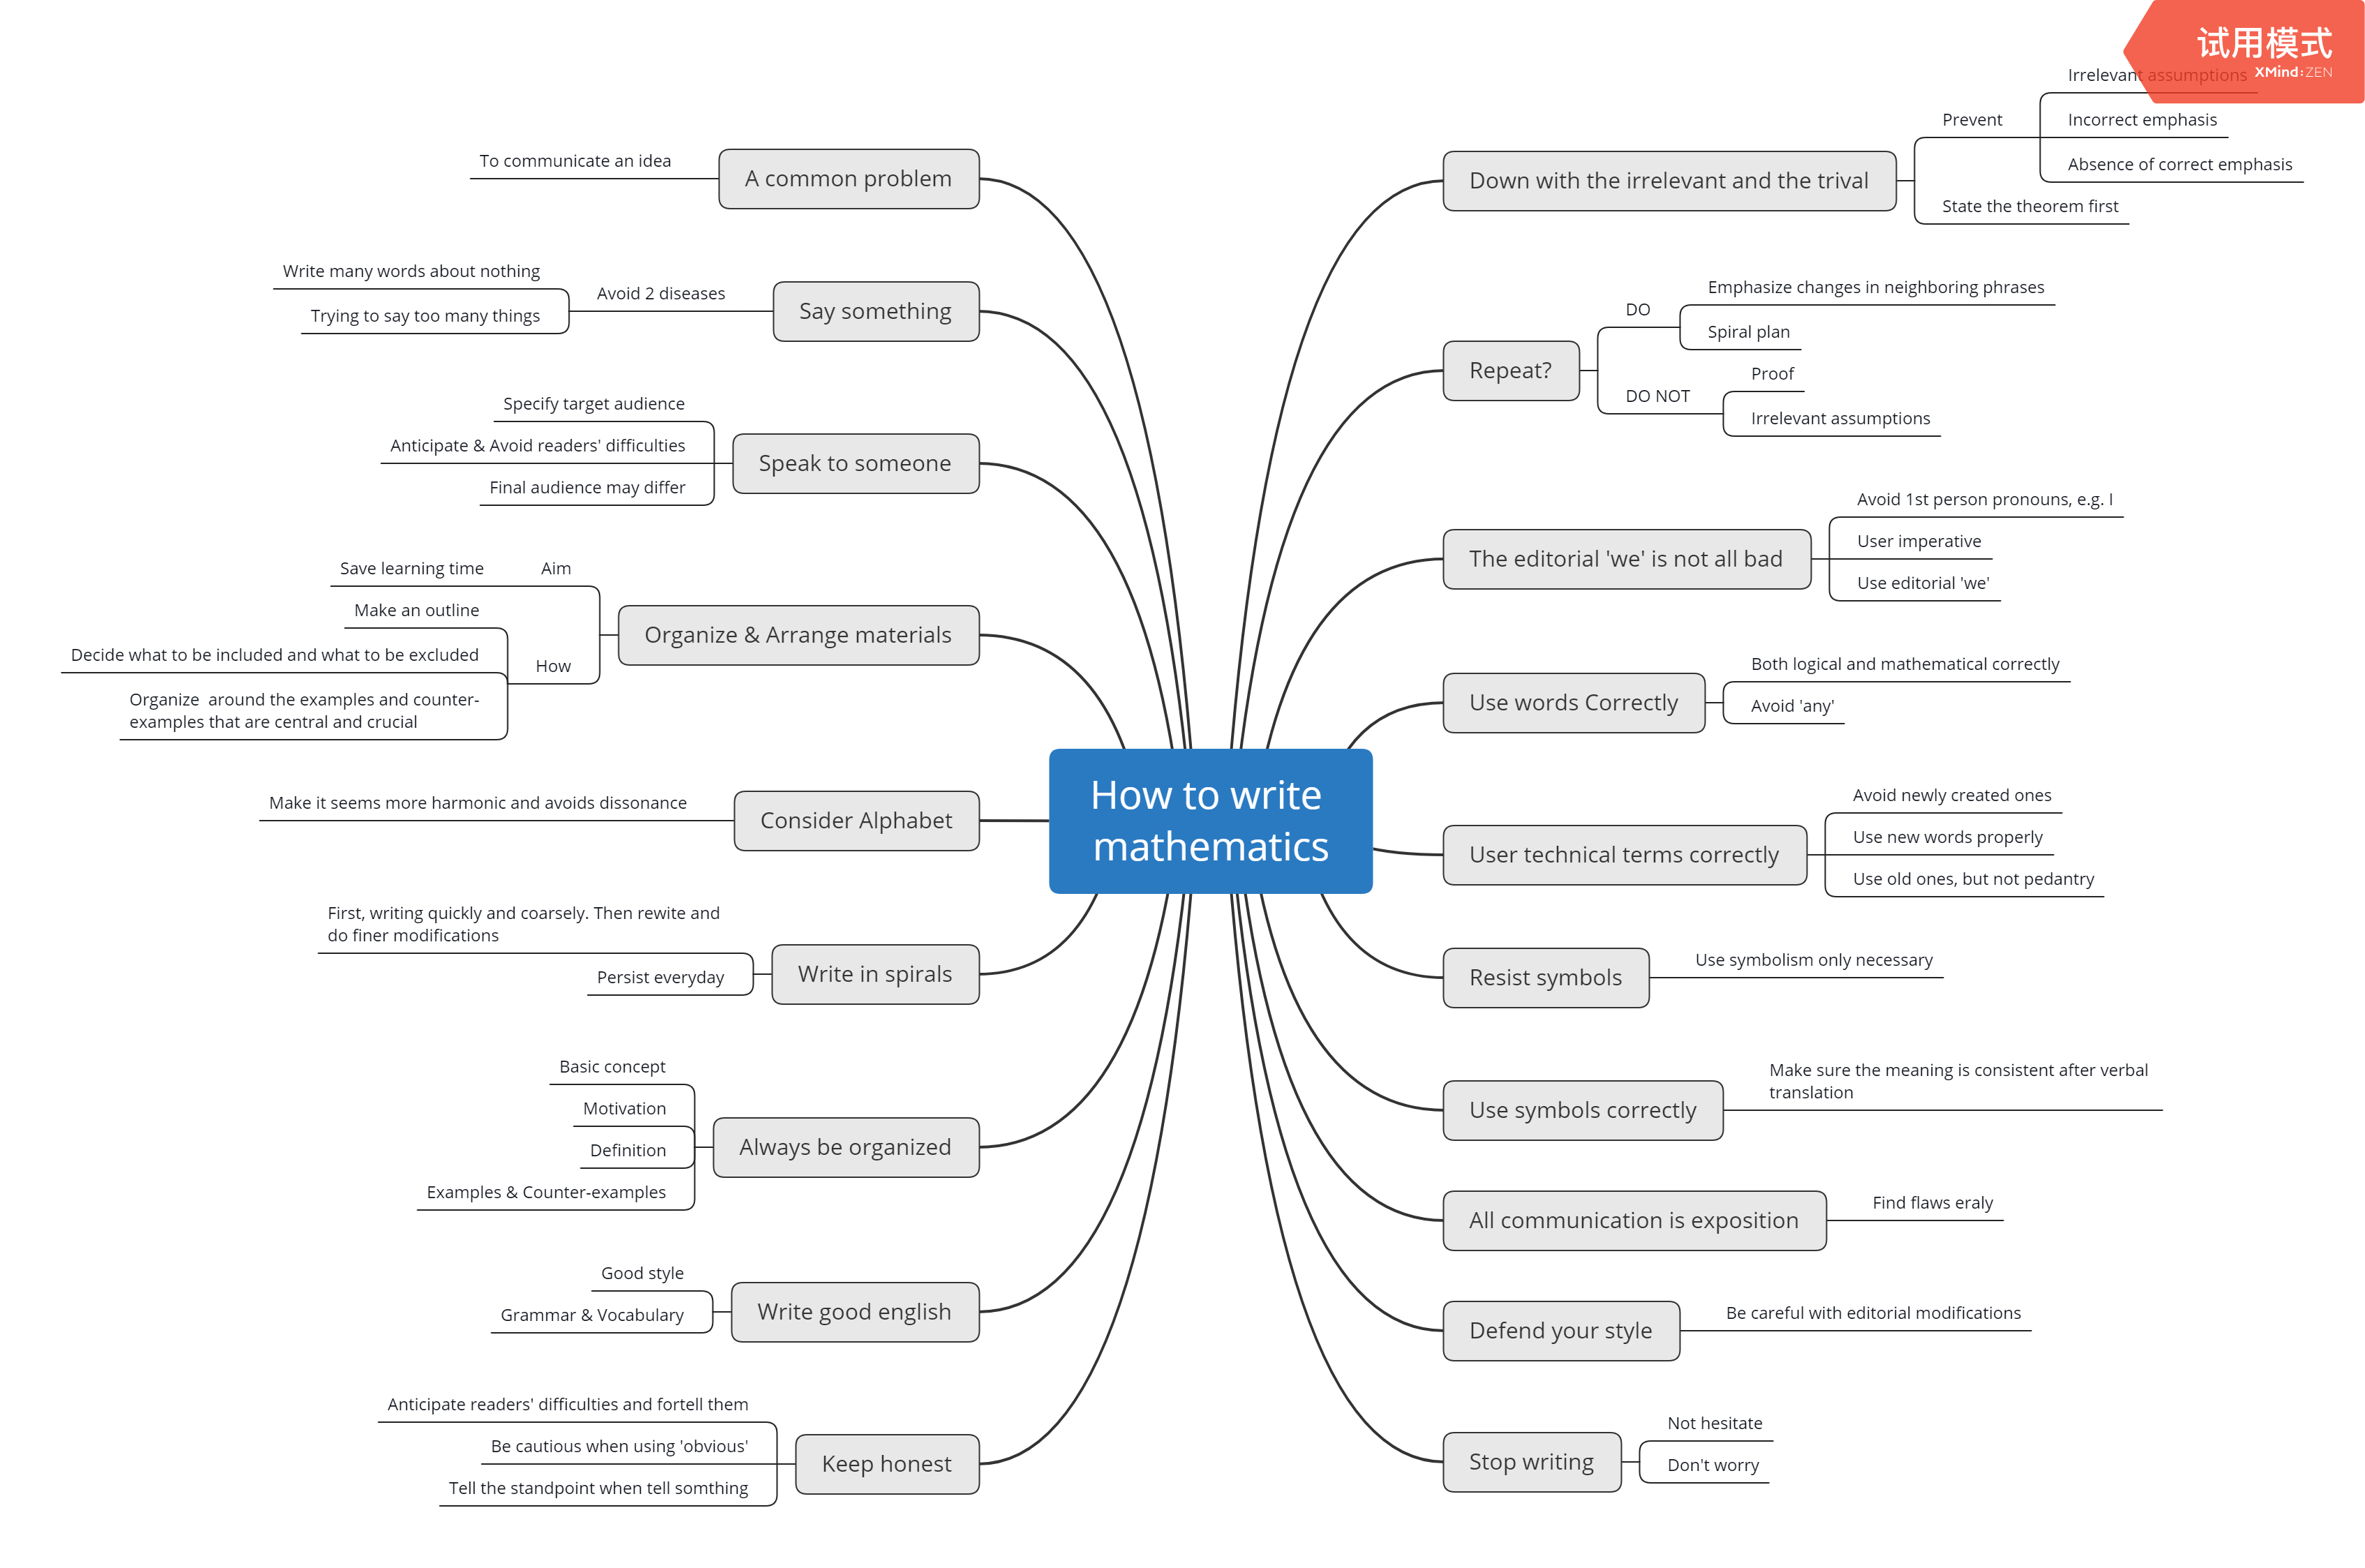
\includegraphics[width=13.5cm]{pic/mind_map.png}
		\caption{How to write mathematics}
		\label{fig:htwm}
	\end{figure}


\section{Group Exercise}
	All the comments and discussions have been submitted to our team leader. Please see Rui Gao's work.
	
\section{Writting skills}
	\begin{enumerate}
		\item 
			``\textbf{Just act naturally}'': `naturally' is not suitable to be adverb for `act'.\newline
			``\textbf{Please give your unbiased opinion}'': No objective in this sentence.\newline
			``\textbf{I need an exact estimate by Friday}'': The two words: `exact' and `estimate' contradict with each other.

		\item 
			Before the agent was \sout{completely} able to \sout{finish} explain\sout{ing} the \sout{various} differences between \sout{all of} the \sout{many} outdoor event packages her company was offering, the customer changed his \sout{future} plans.
	\end{enumerate}

\section{\LaTeX}
	See next page.
	\includepdf[pages=2]{assignment.pdf}

\end{document}